\documentclass[12pt]{article}
\usepackage{amsmath}
\usepackage{amsfonts}
\usepackage{fancyhdr}
\usepackage{titlesec}
\usepackage[margin=1in]{geometry}
\usepackage{siunitx}
\usepackage{booktabs}
\usepackage{graphicx}

\pagestyle{fancy}
\lhead{} 
\chead{} 
\rhead{\thepage} 
\lfoot{} 
\cfoot{} 
\rfoot{} 
\renewcommand{\headrulewidth}{0pt} 
\renewcommand{\footrulewidth}{0pt} 
%\titleformat{\section}[block]{\Large\bfseries\filcenter}{}{1em}{}
%\titleformat{\subsection}[block]{\large\bfseries\filcenter}{}{1em}{}
%To make sure we actually have header 0.5in away from top edge
%12pt is one-sixth of an inch. Subtract this from 0.5in to get headsep value
\setlength\headsep{0.333in}
\pagestyle{fancy}
\linespread{1.4}

\newcommand{\boldrule}{\rule{\linewidth}{2pt}} % Draws a thick line

\newcommand{\overbar}[1]{\mkern 1.5mu\overline{\mkern-1.5mu#1\mkern-1.5mu}\mkern 1.5mu} % Reduces length of \overline


\graphicspath{{Graphics/}}

\begin{document}

\thispagestyle{empty}
\newpage
\vspace*{3cm}
\begin{center}
%Lab title goes here
{\Huge EE 648 -- VLSI Design\\[.5cm]
Binary Coded Hexadecimal for a 7 Segment Display}
\end{center}
\vspace{5mm}
\boldrule\\
\begin{center}

\includegraphics{uaflogo.png}\\[.5cm]
\boldrule\\[3cm]
{\Large
<<<<<<< HEAD
\textsc{Ryker Dial}\\
\textsc{Cody Gossel}\\
\textsc{Zach Krehlik}\\[1cm]
May 1, 2015
=======
Ryker \textsc{Dial}\\
Cody \textsc{Gossel}\\
Zach \textsc{Krehlik}\\[1cm]
February 17, 2017
>>>>>>> e20f97229025155d15eaa7a3f5481cd182cff6a6
}
\end{center}
\pagenumbering{gobble}


\newpage

\thispagestyle{empty}
\tableofcontents

\newpage
<<<<<<< HEAD

\setcounter{page}{1}
=======
\pagenumbering{arabic}
>>>>>>> e20f97229025155d15eaa7a3f5481cd182cff6a6

%Rest of report goes here
\section{Top Level Design}

\section{Detailed Design}

\begin{figure}[h]
	\centering
	\label{fig:TopLevelCkt}
	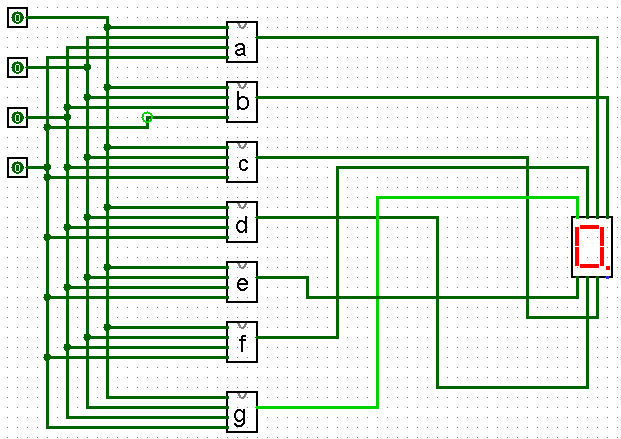
\includegraphics[scale=.8]{topLevelLogicCkt.png}
	\caption{Circuit top level layout}
\end{figure}


\begin{figure}[h]
	\centering
	\label{fig:aBlockGates}
	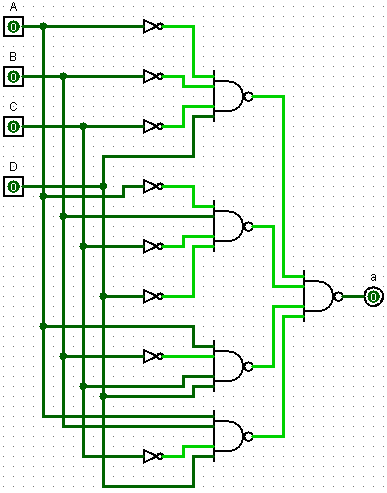
\includegraphics[width=0.65\linewidth, keepaspectratio]{a_logicCkt}
	\caption{Block a Gate Level Schematic}
\end{figure}

\begin{equation}
	a = \overline{\overbar{(\bar{A}\bar{B}\bar{C}D)}\overbar{(\bar{A}B\bar{C}\bar{D})}\overbar{(A\bar{B}CD)}\overbar{(AB\bar{C}D)}}
\end{equation}

\begin{figure}[h]
	\centering
	\label{fig:bBlockGates}
	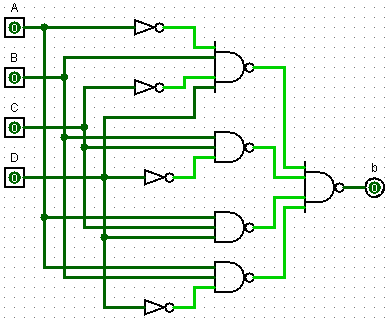
\includegraphics[width=0.65\linewidth, keepaspectratio]{b_logicCkt}
	\caption{Block b Gate Level Schematic}
\end{figure}

\begin{equation}
	b = \overline{\overbar{(\bar{A}B\bar{C}D)}\overbar{(BC\bar{D})}\overbar{(ACD)}\overbar{(AB\bar{D})}}
\end{equation}

\begin{figure}[h]
	\centering
	\label{fig:cBlockGates}
	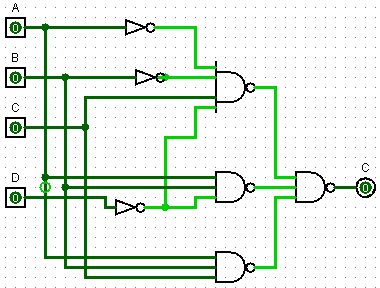
\includegraphics[width=0.65\linewidth, keepaspectratio]{c_logicCkt}
	\caption{Block c Gate Level Schematic}
\end{figure}

\begin{equation}
	c = \overline{\overbar{(\bar{A}\bar{B}C\bar{D})}\overbar{(AB\bar{D})}\overbar{(ABC)}}
\end{equation}

\begin{figure}[h]
	\centering
	\label{fig:dBlockGates}
	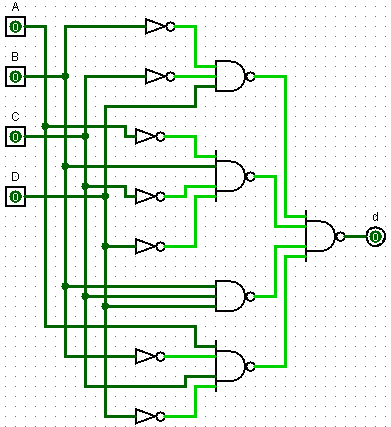
\includegraphics[width=0.65\linewidth, keepaspectratio]{d_logicCkt}
	\caption{Block d Gate Level Schematic}
\end{figure}

\begin{equation}
	d = \overline{\overbar{(\bar{B}\bar{C}D)}\overbar{(\bar{A}B\bar{C}\bar{D})}\overbar{(BCD)}\overbar{A\bar{B}C\bar{D}}}
\end{equation}

\begin{figure}[h]
	\centering
	\label{fig:eBlockGates}
	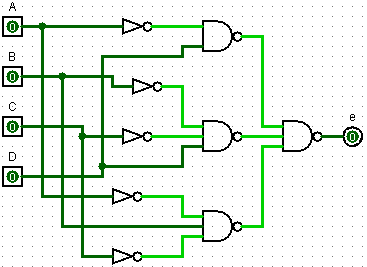
\includegraphics[width=0.65\linewidth, keepaspectratio]{e_logicCkt}
	\caption{Block e Gate Level Schematic}
\end{figure}

\begin{equation}
	e = \overline{\overbar{(\bar{A}D)}\overbar{(\bar{B}\bar{C}D)}\overbar{(\bar{A}B\bar{C})}}
\end{equation}

\begin{figure}[h]
	\centering
	\label{fig:fBlockGates}
	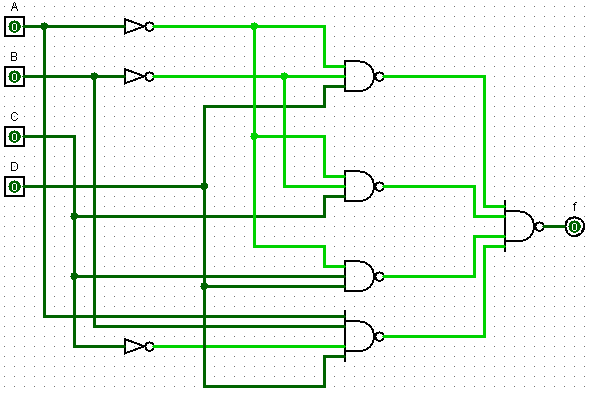
\includegraphics[width=0.65\linewidth, keepaspectratio]{f_logicCkt}
	\caption{Block f Gate Level Schematic}
\end{figure}

\begin{equation}
	f = \overline{\overbar{(\bar{A}\bar{B}D)}\overbar{(\bar{A}\bar{B}C)}\overbar{(\bar{A}CD)}\overbar{(AB\bar{C}D)}}
\end{equation}

\begin{figure}[h]
	\centering
	\label{fig:gBlockGates}
	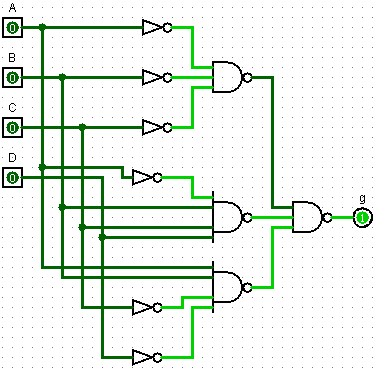
\includegraphics[width=0.65\linewidth, keepaspectratio]{g_logicCkt}
	\caption{Block g Gate Level Schematic}
\end{figure}

\begin{equation}
	g = \overline{\overbar{(\bar{A}\bar{B}\bar{C})}\overbar{(\bar{A}BCD)}\overbar{(AB\bar{C}\bar{D})}}
\end{equation}

\end{document}
